\chapter{Introduction}
\label{chap:introduction}

QMCPACK is an open-source, high-performance electronic structure code
that implements numerous Quantum Monte Carlo (QMC) algorithms. Its main
applications are electronic structure calculations of molecular,
periodic 2D, and periodic 3D solid-state systems. Variational Monte
Carlo (VMC), diffusion Monte Carlo (DMC), and a number of other
advanced QMC algorithms are implemented. By directly solving the
Schrodinger equation, QMC methods offer greater accuracy than methods
such as density functional theory but at a trade-off of much greater
computational expense. Distinct from many other correlated many-body
methods, QMC methods are readily applicable to both bulk
(periodic) and isolated molecular systems.

QMCPACK is written in C++ and is designed with the modularity afforded by
object-oriented programming. It makes extensive use of template
metaprogramming to achieve high computational efficiency. Because of the
modular architecture, the addition of new wavefunctions, algorithms,
and observables is relatively straightforward. For parallelization,
QMCPACK uses a fully hybrid (OpenMP,CUDA)/MPI approach to optimize
memory usage and to take advantage of the growing number of cores per
SMP node or graphical processing units (GPUs) and accelerators. High
parallel and computational efficiencies are achievable on the largest
supercomputers. Finally, QMCPACK uses standard file formats for
input and output in XML and HDF5 to facilitate data exchange.

This manual currently serves as an introduction to the essential features
of QMCPACK and as a guide to installing and running it. Over time this
manual will be expanded to include a fuller introduction to QMC
methods in general and to include more of the specialized features in
QMCPACK.
%Test of the bibliography\cite{CeperleyAlderPRL1980}.

\section{Quickstart and a first QMCPACK calculation}
In case you are keen to get started, this section describes how to quickly
build and run QMCPACK on a standard UNIX or Linux-like system. The
autoconfiguring build system usually works without much fuss on these
systems.  If C++, MPI, BLAS/LAPACK, FFTW, HDF5, and CMake are already
installed, QMCPACK can be built and run within five minutes. For
supercomputers, cross-compilation systems, and other computer clusters,
the build system might require hints on the locations of libraries and
which versions to use, typical of any code; see Chapter
\ref{chap:obtaininginstalling}. Section~\ref{sec:installexamples}
includes complete examples of installations for common workstations and supercomputers that you can reuse.

To build QMCPACK:

\begin{enumerate}
\item Download the latest QMCPACK distribution from
  \url{http://www.qmcpack.org}.
\item Untar the archive (e.g., \ishell{tar xvf
    qmcpack\_v1.3.tar.gz}).
\item Check the instructions in the README file.
\item Run CMake in a suitable build directory to configure QMCPACK for
  your system: \ishell{cd qmcpack/build; cmake ..}
\item If CMake is unable to find all needed libraries, see Chapter
  \ref{chap:obtaininginstalling} for instructions and specific build
  instructions for common systems.
\item Build QMCPACK: \ishell{make} or \ishell{make -j 16}; use the latter
  for a faster parallel build on a system using, for example, 16 processes.
\item The QMCPACK executable is \ishell{bin/qmcpack}.
\end{enumerate}

QMCPACK is distributed with examples illustrating different
capabilities. Most of the examples are designed to run quickly with
modest resources. We'll run a short diffusion Monte Carlo calculation
of a water molecule:

\begin{enumerate}
\item Go to the appropriate example directory: \ishell{cd
    ../examples/molecules/H2O}.
\item (Optional) Put the QMCPACK binary on your path:\\ \ishell{export PATH=\$PATH:location-of-qmcpack/build/bin}.
\item Run QMCPACK: \ishell{../../../build/bin/qmcpack simple-H2O.xml} or
  \ishell{qmcpack simple-H2O.xml} if you followed the step above.
\item The run will output to the screen and generate a number of files:
\begin{verbatim}
$ls H2O*
H2O.HF.wfs.xml      H2O.s001.scalar.dat H2O.s002.cont.xml
H2O.s002.qmc.xml    H2O.s002.stat.h5    H2O.s001.qmc.xml
H2O.s001.stat.h5    H2O.s002.dmc.dat    H2O.s002.scalar.dat
\end{verbatim}
\item Partially summarized results are in the standard text files with the
  suffixes scalar.dat and dmc.dat. They are viewable with any standard editor.
\end{enumerate}

If you have Python and matplotlib installed, you can use the
\ishell{qmca} analysis utility to produce statistics and plots of the
data. See Chapter~\ref{chap:analyzing} for information on analyzing
QMCPACK data.
\begin{verbatim}
export PATH=$PATH:location-of-qmcpack/nexus/bin 
export PYTHONPATH=$PYTHONPATH:location-of-qmcpack/nexus/library
qmca H2O.s002.scalar.dat         # For statistical analysis of the DMC data
qmca -t -q e H2O.s002.scalar.dat # Graphical plot of DMC energy
\end{verbatim}

The last command will produce a graph as per
Fig.~\ref{fig:quick_qmca_dmc_trace}. This shows the average energy of
the DMC walkers at each timestep. In a real simulation we would have
to check equilibration, convergence with walker population, time step, etc.

Congratulations, you have completed a DMC calculation with QMCPACK!

\begin{figure}
  \centering
  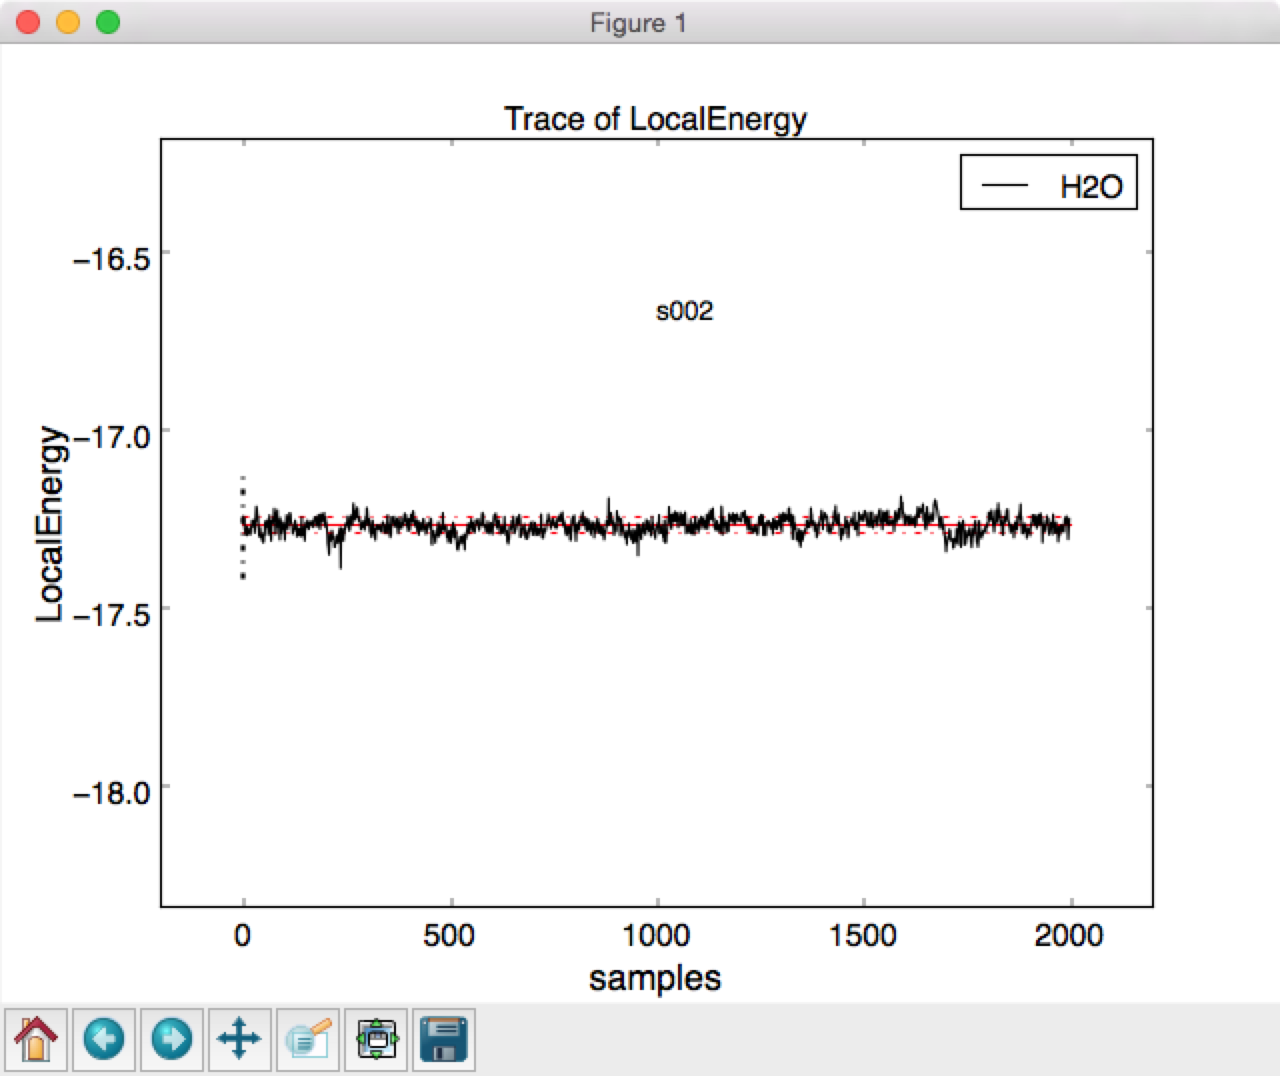
\includegraphics[width=10cm]{./figures/quick_qmca_dmc_trace.png}
  \caption{Trace of walker energies produced by the qmca tool for a simple
    water molecule example.}
  \label{fig:quick_qmca_dmc_trace}
\end{figure}

\section{Authors and History}
\label{sec:history}
QMCPACK was initially written by Jeongnim Kim while in the group of
Professor David Ceperley at the University of Illinois at
Urbana-Champaign, with later contributations being made at Oak Ridge National Laboratory (ORNL). Over the years, many others have contributed, particularly
students and researchers in the groups of Professor David Ceperley
and Professor Richard M. Martin, as well as staff at Lawrence Livermore
National Laboratory, Sandia National Laboratories, Argonne National
Laboratory, and ORNL.

Additional developers, contributors, and advisors include
Anouar Benali,
Mark A. Berrill,  
David M. Ceperley, 
Simone Chiesa,
Raymond C. III Clay,
Bryan Clark,
Kris T. Delaney,
Kenneth P. Esler,
Paul R. C. Kent,
Jaron T. Krogel,
Ying Wai Li,
Ye Luo,
Jeremy McMinis,
Miguel A. Morales,
William D. Parker,
Nichols A. Romero,
Luke Shulenburger,
Norman M. Tubman,
and Jordan E. Vincent.

If you should be added to this list, please let us know.

Development of QMCPACK has been supported financially by
several grants, including the following:

\begin{itemize}
\item ``Network for ab initio many-body methods: development, education
  and training'' supported through the Predictive
  Theory and Modeling for Materials and Chemical Science program by
  the U.S. Department of Energy Office of Science, Basic Energy
  Sciences
\item ``QMC Endstation,'' supported by Accelerating Delivery of Petascale
  Computing Environment at the DOE Leadership Computing Facility at
  ORNL
\item PetaApps, supported by the US National Science
  Foundation
\item Materials Computation Center (MCC), supported by the
  US National Science Foundation
\end{itemize}


\section{Support and Contacting the Developers}
\label{sec:support}

Questions about installing, applying, or extending QMCPACK can be
posted on the QMCPACK Google group at
\url{https://groups.google.com/forum/#!forum/qmcpack}. You may also
email any of the developers, but we recommend checking the group
first. Particular attention is given to any problem reports.

\section{Performance}
\label{sec:performance}

QMCPACK implements modern Monte Carlo (MC) algorithms, is highly parallel,
and is written using very efficient code for high per-CPU or on-node performance. In particular, the code is highly vectorizable,
giving high performance on modern central processing units (CPUs) and GPUs. We believe QMCPACK
delivers performance either comparable to or better than other QMC
codes when similar calculations are run, particularly for the most
common QMC methods and for large systems. If you find a calculation where this is not the
case, or you simply find performance slower than expected, please post on the Google
group or contact one of the developers. These reports are valuable. If your calculation is
sufficiently mainstream we will optimize QMCPACK to improve
the performance.

\section{Open source license}
\label{sec:license}

QMCPACK is distributed under the University of Illinois at
Urbana-Champaign/National Center for Supercomputing Applications (UIUC/NCSA) Open
Source License. 

\begin{verbatim}
		  University of Illinois/NCSA Open Source License

Copyright (c) 2003, University of Illinois Board of Trustees.
All rights reserved.

Developed by:   
  Jeongnim Kim
  Condensed Matter Physics,
  National Center for Supercomputing Applications, University of Illinois
  Materials computation Center, University of Illinois
  http://www.mcc.uiuc.edu/qmc/

Permission is hereby granted, free of charge, to any person obtaining a
copy of this software and associated documentation files (the
``Software''), to deal with the Software without restriction, including
without limitation the rights to use, copy, modify, merge, publish,
distribute, sublicense, and/or sell copies of the Software, and to
permit persons to whom the Software is furnished to do so, subject to
the following conditions:

        * Redistributions of source code must retain the above copyright 
          notice, this list of conditions and the following disclaimers.
        * Redistributions in binary form must reproduce the above copyright 
          notice, this list of conditions and the following disclaimers in 
          the documentation and/or other materials provided with the 
          distribution.
        * Neither the names of the NCSA, the MCC, the University of Illinois, 
          nor the names of its contributors may be used to endorse or promote 
          products derived from this Software without specific prior written 
          permission.

THE SOFTWARE IS PROVIDED "AS IS", WITHOUT WARRANTY OF ANY KIND, EXPRESS
OR IMPLIED, INCLUDING BUT NOT LIMITED TO THE WARRANTIES OF MERCHANTABILITY, 
FITNESS FOR A PARTICULAR PURPOSE AND NONINFRINGEMENT. IN NO EVENT SHALL 
THE CONTRIBUTORS OR COPYRIGHT HOLDERS BE LIABLE FOR ANY CLAIM, DAMAGES OR 
OTHER LIABILITY, WHETHER IN AN ACTION OF CONTRACT, TORT OR OTHERWISE, 
ARISING FROM, OUT OF OR IN CONNECTION WITH THE SOFTWARE OR THE USE OR 
OTHER DEALINGS WITH THE SOFTWARE.
\end{verbatim}

Copyright is generally believed to remain with the authors of the
individual sections of code. See the various notations in the source code as
well as the code history.

\section{Contributing to QMCPACK}
\label{sec:contributing}

QMCPACK is fully open source, and we welcome contributions. If you are
planning a development, early discussions are encouraged. Please
post on the QMCPACK Google group or contact the developers. We can tell you whether anyone else is working on a similar feature or whether
any related work has been done in the past.  Credit for your
contribution can be obtained, for example, through citation of a paper or by
becoming one of the authors on the next version of the standard
QMCPACK reference citation.

A guide to developing for QMCPACK, including instructions on how to
work with GitHub and make pull requests (contributions) to the main
source are listed on the QMCPACK GitHub wiki:
\url{https://github.com/QMCPACK/qmcpack/wiki}.

Contributions are made under the same license as QMCPACK, the
UIUC/NCSA open source license. If this is problematic, please discuss
with a developer.

Please note the following guidelines for contributions:
\begin{itemize}
\item Additions should be fully synchronized with the latest release
  version and ideally the latest develop branch on github. Merging of code
  developed on older versions is error prone.
\item Code should be cleanly formatted, commented, portable, and accessible to
  other programmers. That is, if you need to use any clever tricks, add a comment
  to note this, why the trick is needed, how it works, etc. Although we like
  high performance, ease of maintenance and accessibility are also
  considerations.
\item Comment your code. You are not only writing it for the compiler
  for also for other humans! (We know this is a repeat of the previous
  point, but it is important enough to repeat.)
\item Write a brief description of the method, algorithms, and inputs and outputs
  suitable for inclusion in this manual.
\item Develop some short tests that exercise the
  functionality that can be used for validation and for examples. We
  can help with this and their integration into the test system.
\end{itemize}

\section{QMCPACK Roadmap}
\label{sec:roadmap}

A general outline of the QMCPACK roadmap is given in Sections 1.7.1 and 1.7.2 . Suggestions
for improvements are welcome, particularly those that would facilitate new
scientific applications. For example, if an interface to a particular
quantum chemical or density functional code would help, this would be
given strong consideration.

\subsection{Code}

We will continue to improve the accessibility and usability of
QMCPACK through combinations of more convenient input parameters, improved
workflow, integration with more quantum chemical and density
functional codes, and a wider range of examples.

In terms of methodological development, we expect to significantly
increase the range of QMC algorithms in QMCPACK in the near future.

Computationally, we are porting QMCPACK to the next generation of
supercomputer systems. The internal changes required to run efficiently on these
systems are expected to benefit \emph{all} platforms due
to improved vectorization, cache utilization, and memory performance.

\subsection{Documentation}

This manual describes the core features of QMCPACK that are
required for routine research calculations, i.e., the VMC and DMC
methods, how to obtain and optimize trial wavefunctions, and simple
observables. Over time this manual will be expanded to include a
broader introduction to QMC methods and to describe more features of
the code.

Because of its history as a research code, QMCPACK contains a variety of
additional QMC methods, trial wavefunction forms, potentials, etc.,
that, although not critical, might be very useful for specialized
calculations or particular material or chemical systems. These
``secret features'' (every code has these) are not actually secret but
simply lack descriptions, example inputs, and tests. You are
encouraged to browse and read the source code to find them. New
descriptions will be added over time but can also be prioritized and
added on request (e.g., if a specialized Jastrow factor would help or
a historical Jastrow form is needed for benchmarking).


